
% This LaTeX was auto-generated from MATLAB code.
% To make changes, update the MATLAB code and republish this document.

\documentclass{article}
\usepackage{graphicx}
\usepackage{color}

\sloppy
\definecolor{lightgray}{gray}{0.5}
\setlength{\parindent}{0pt}

\begin{document}

    
    
\subsection*{Contents}

\begin{itemize}
\setlength{\itemsep}{-1ex}
   \item Final Problem 4
   \item A. Generate the population of Gamma RVs
   \item B Part 1: Create Sample Distributions of Size n
\end{itemize}


\subsection*{Final Problem 4}

\begin{par}
Taylor Bodin 9 Dec 2016
\end{par} \vspace{1em}
\begin{verbatim}
% Setup Variables
clear; close all; clc;
set(0,'DefaultFigureWindowStyle','docked')

N = 500000; %Number of RV in the population
num_bins = 50; %Standard number of bins for histograms
n = [10 20 40 80 100 200 500];
ci = .975;
\end{verbatim}


\subsection*{A. Generate the population of Gamma RVs}

\begin{verbatim}
pop = random('Gamma',1,1,[1,N]);

% Descripitive Stats
mu = mean(pop); % Given
var = std(pop)^2;
skew = skewness(pop);
pop_quant_upper = quantile(pop,ci);
pop_quant_lower = quantile(pop,1-ci);

pop_stat_str = {['\mu = ', num2str(mu)];
    ['\sigma^2 = ' num2str(var)];
    ['Skew = ' num2str(skew)];
    ['Upper Quantile: ' num2str(pop_quant_upper)];
    ['Lower Quantile: ' num2str(pop_quant_lower)]};


% Population Figure
f1 = figure(1);

% Histogram
pop_hist = histogram(pop);
pop_hist.Normalization = 'PDF';
pop_hist.NumBins = num_bins;

% Quantiles
line([pop_quant_lower pop_quant_lower], get(gca, 'ylim'),...
    'Color', 'Red', 'LineWidth', 2, 'LineStyle', '--');
line([pop_quant_upper pop_quant_upper], get(gca, 'ylim'),...
    'Color', 'Green', 'LineWidth', 2, 'LineStyle', '--');

% Annotation
dim = [.4 .3 .3 .3];
annotation('textbox',dim,'String',pop_stat_str,'FitBoxToText','on');

% Figure Properties
title('Simulated PDF of the Gamma(1,1) RV')
xlabel('RV value');
f1.CurrentAxes.XAxis.Limits = [0 4];
ylabel('Probability Density');
legend('Gamma(1,1) PDF', 'Lower Quantile (.025)', 'Upper Quantile (.975)');
\end{verbatim}

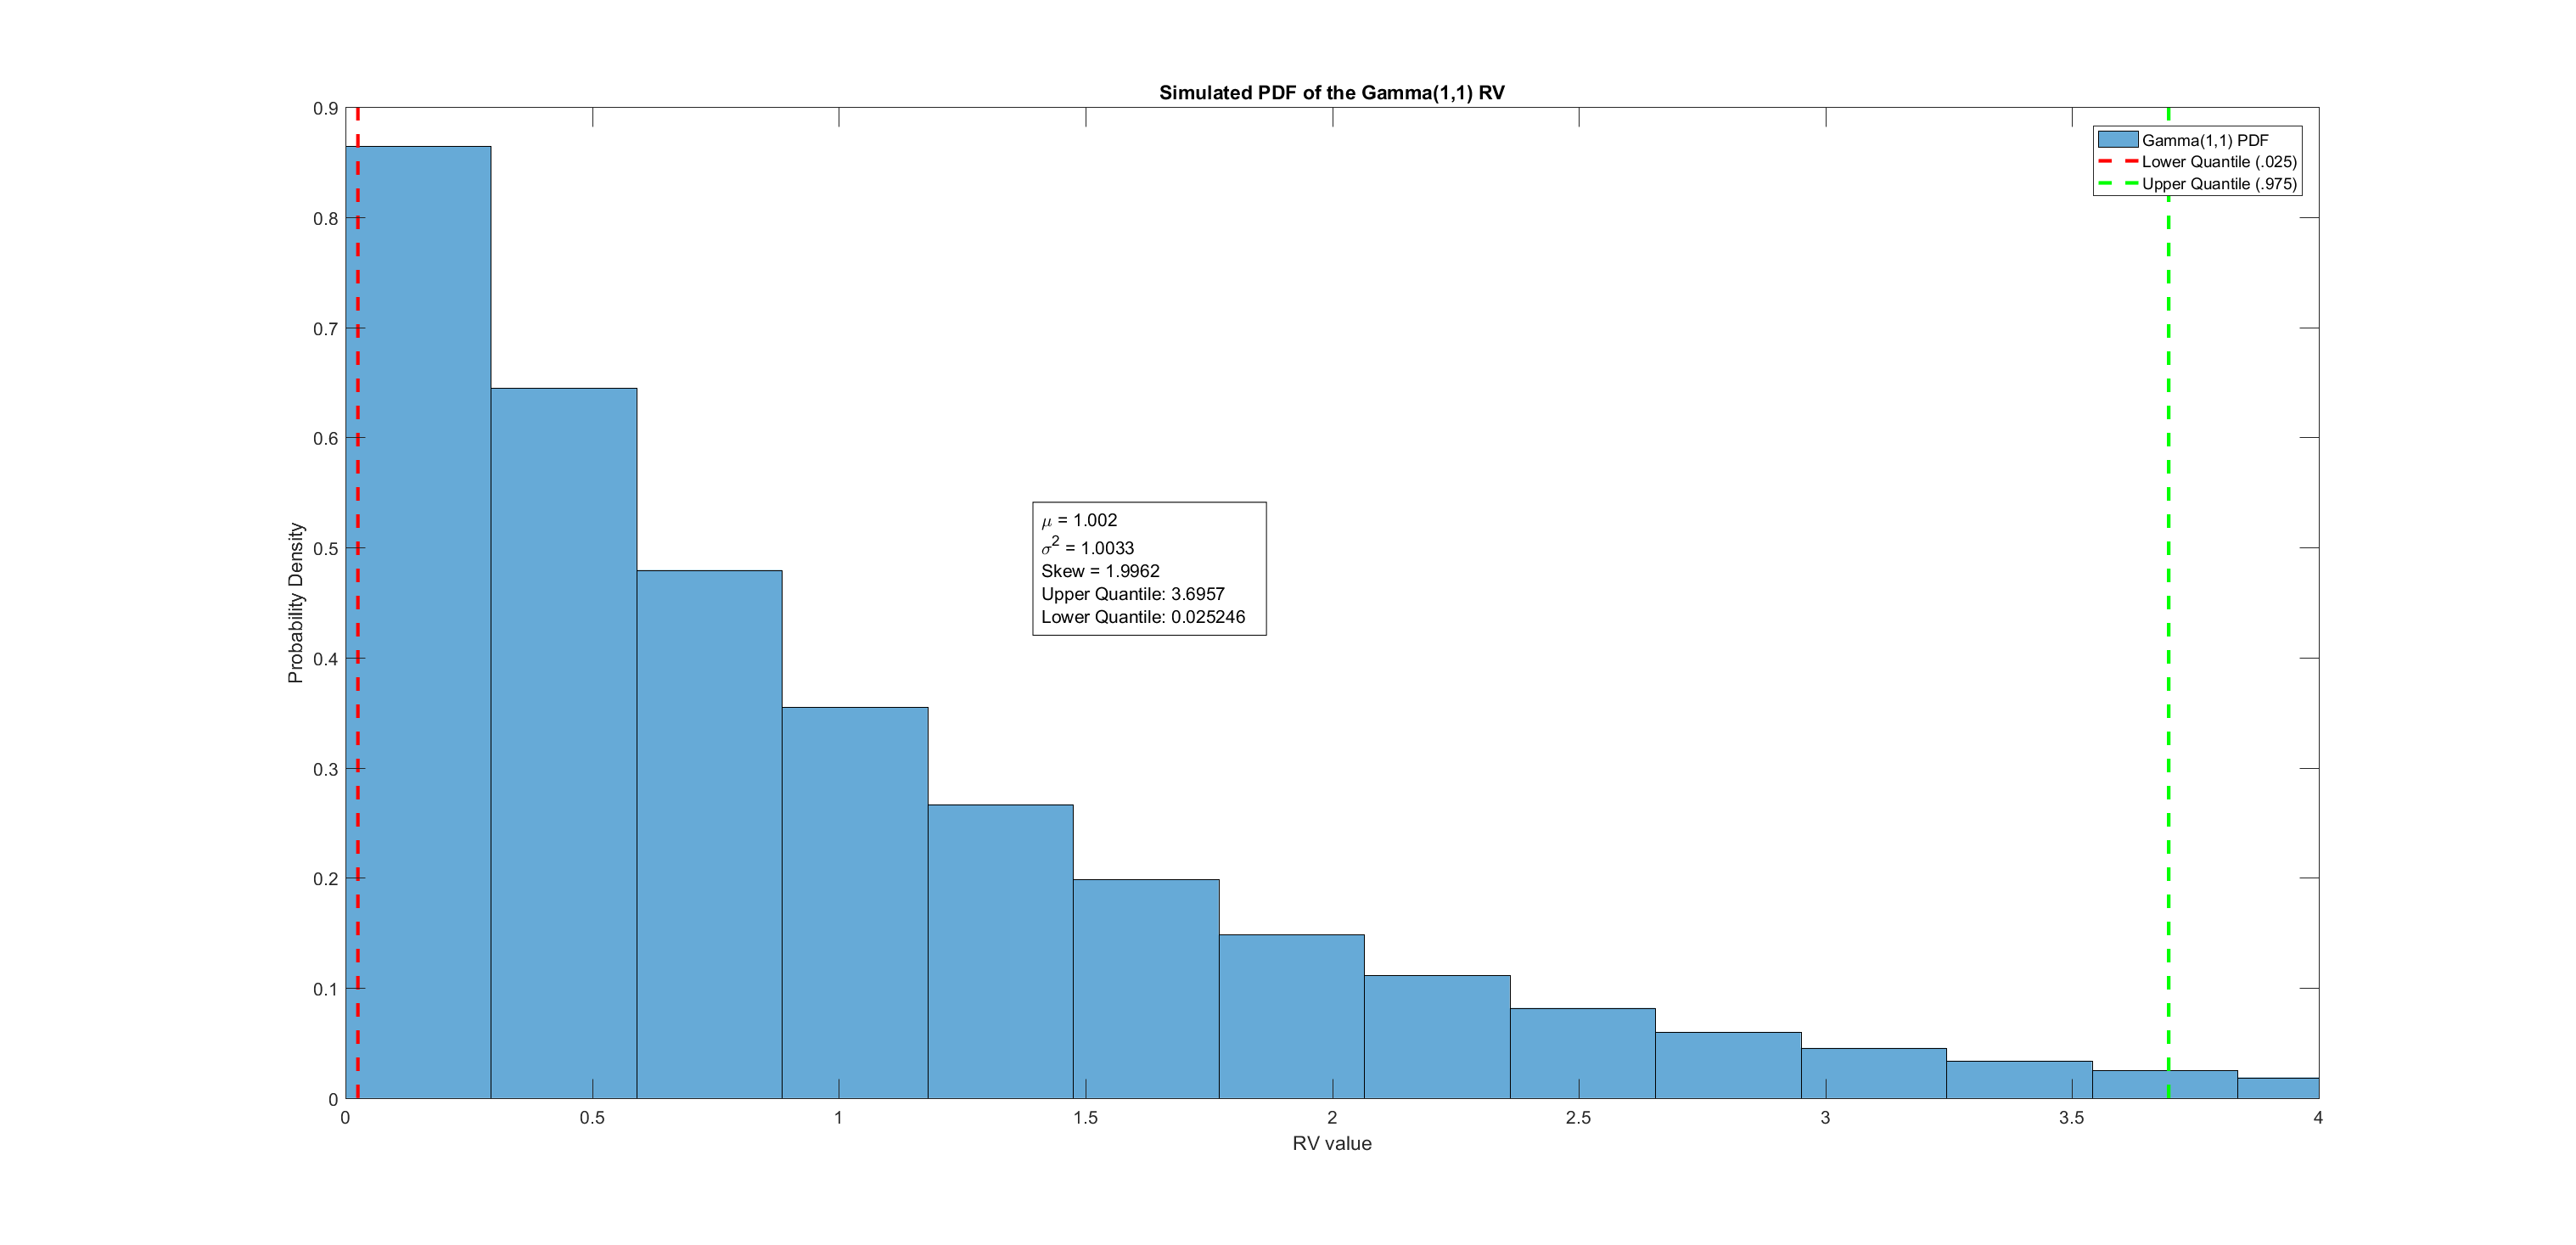
\includegraphics [width=4in]{prob4_01.eps}


\subsection*{B Part 1: Create Sample Distributions of Size n}

\begin{verbatim}
for k=1:length(n)

sample = reshape(pop,n(k),[]);
sample = sample(:,1:1000); % Per the instructions only want 1000

% Descriptive Stats
s_mu = mean(sample);
mu_var = mean(std(s_mu).^2);
mu_skew = mean(skewness(s_mu));
s_quant_upper = mean(quantile(s_mu,ci));
s_quant_lower = mean(quantile(s_mu,1-ci));
ci_upper = mean(s_mu + sqrt(var/n(k))*qfuncinv((1-ci)/2));
ci_lower = mean(s_mu - sqrt(var/n(k))*qfuncinv((1-ci)/2));

% Summary of Descriptive Stats
s_stat_str = {['\mu = ', num2str(mean(s_mu))];
    ['\sigma^2 = ' num2str(mu_var)];
    ['Skew = ' num2str(mu_skew)];
    ['Upper Quantile: ' num2str(s_quant_upper)];
    ['Lower Quantile: ' num2str(s_quant_lower)];
    ['Upper Confidence Interval: ' num2str(ci_upper)];
    ['Lower Confidence Interval: ' num2str(ci_lower)]};

% Central Limit Theorem Approximation
cl_pd = makedist('Normal', 'mu', mu, 'sigma', var/sqrt(n(k)));
range = 0:.01:2.5;
cl_pdf = pdf(cl_pd,range);

% Create the figure
f2 = figure(k+1);
hold on
% -- Mean Histogram
s_hist = histogram(s_mu);
s_hist.Normalization = 'PDF';
s_hist.NumBins = num_bins;

xlims = f2.CurrentAxes.XAxis.Limits; %Need these xlims scaled for the hist

% -- Quantiles
q1 = line([s_quant_lower s_quant_lower], get(gca, 'ylim'),...
    'Color', 'Green', 'LineWidth', 2, 'LineStyle', '--');
q2 = line([s_quant_upper s_quant_upper], get(gca, 'ylim'),...
    'Color', 'Green', 'LineWidth', 2, 'LineStyle', '--');

% -- Central Limit Approximation
p1 = plot(range,cl_pdf, 'LineWidth', 2, 'LineStyle', '-.');

% -- Confidence Intervals
ci_1 = line([ci_lower ci_lower], get(gca, 'ylim'),...
    'Color', 'Red', 'LineWidth', 2, 'LineStyle', '--');
ci_2 = line([ci_upper ci_upper], get(gca, 'ylim'),...
    'Color', 'Red', 'LineWidth', 2, 'LineStyle', '--');

% -- Descripitve Annotation
dim = [.815 .52 .3 .3];
a1 = annotation('textbox',dim,'String',s_stat_str,'FitBoxToText','on');

% -- Figure Properties
f2.CurrentAxes.XAxis.Limits = xlims;
title(['PDF of Sample Means of Sample Size ' num2str(n(k))])
xlabel('Value of \mu');
ylabel('Probability Density');
legend([s_hist q1 p1 ci_1], ...
    ['PDF of \mu_{N=' num2str(n(k)) '}'], '97.5% Quantiles'...
    ,'Central Limit Approximation', '97.5% Confidence Intervals');
hold off
end
\end{verbatim}

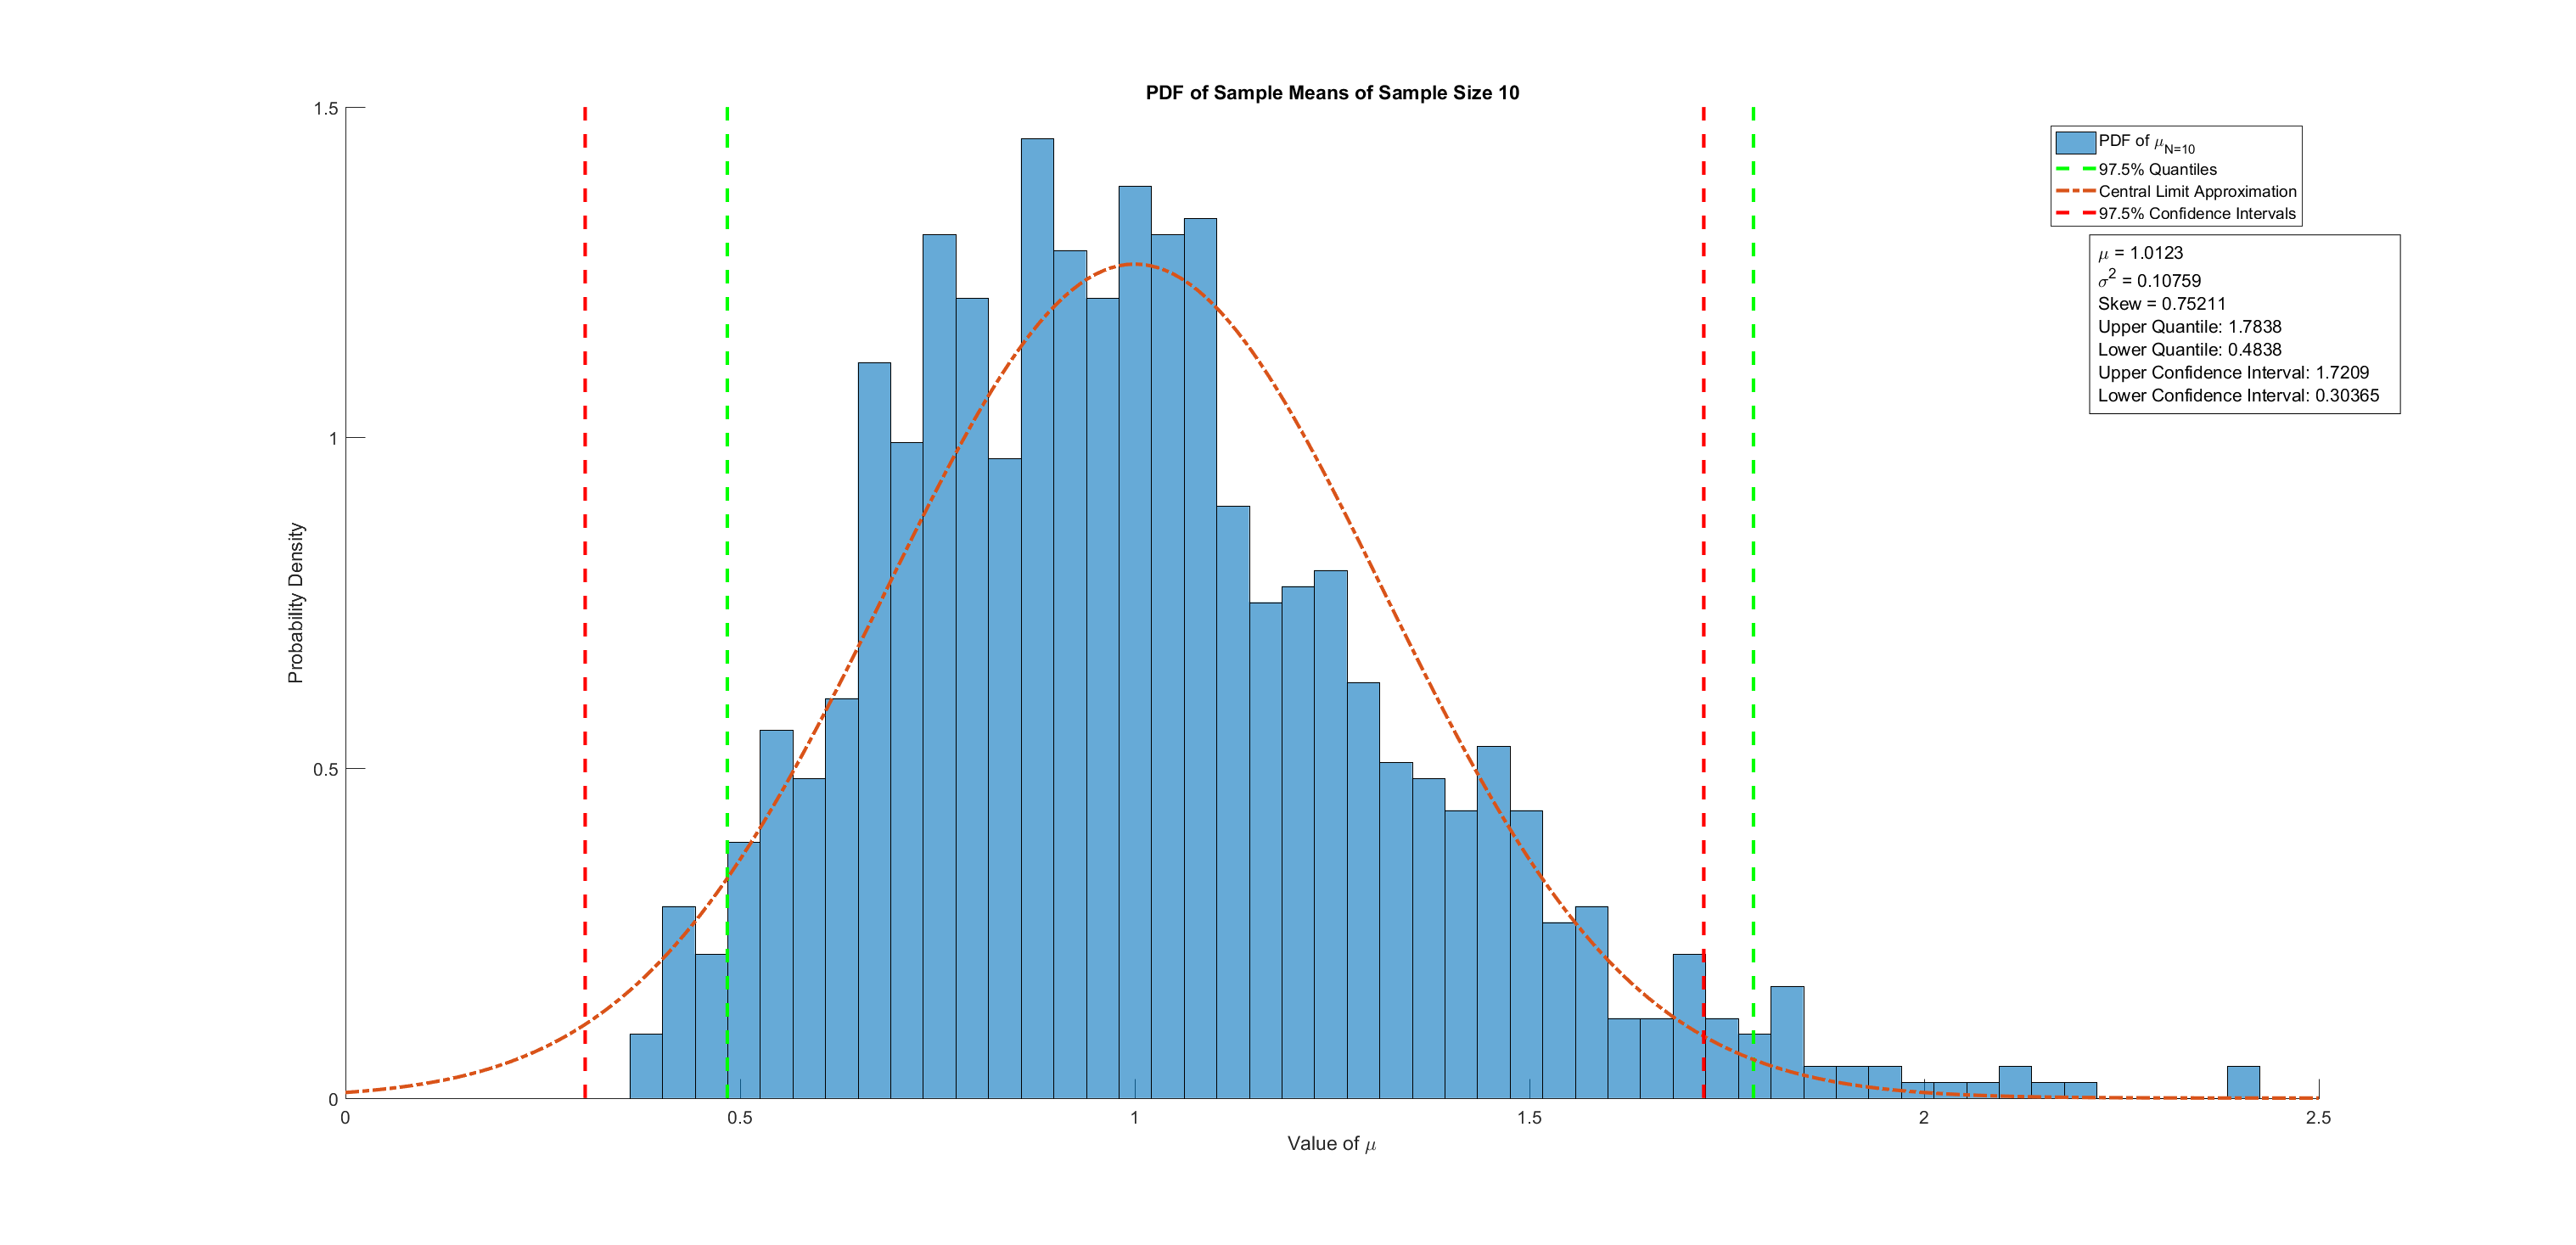
\includegraphics [width=4in]{prob4_02.eps}

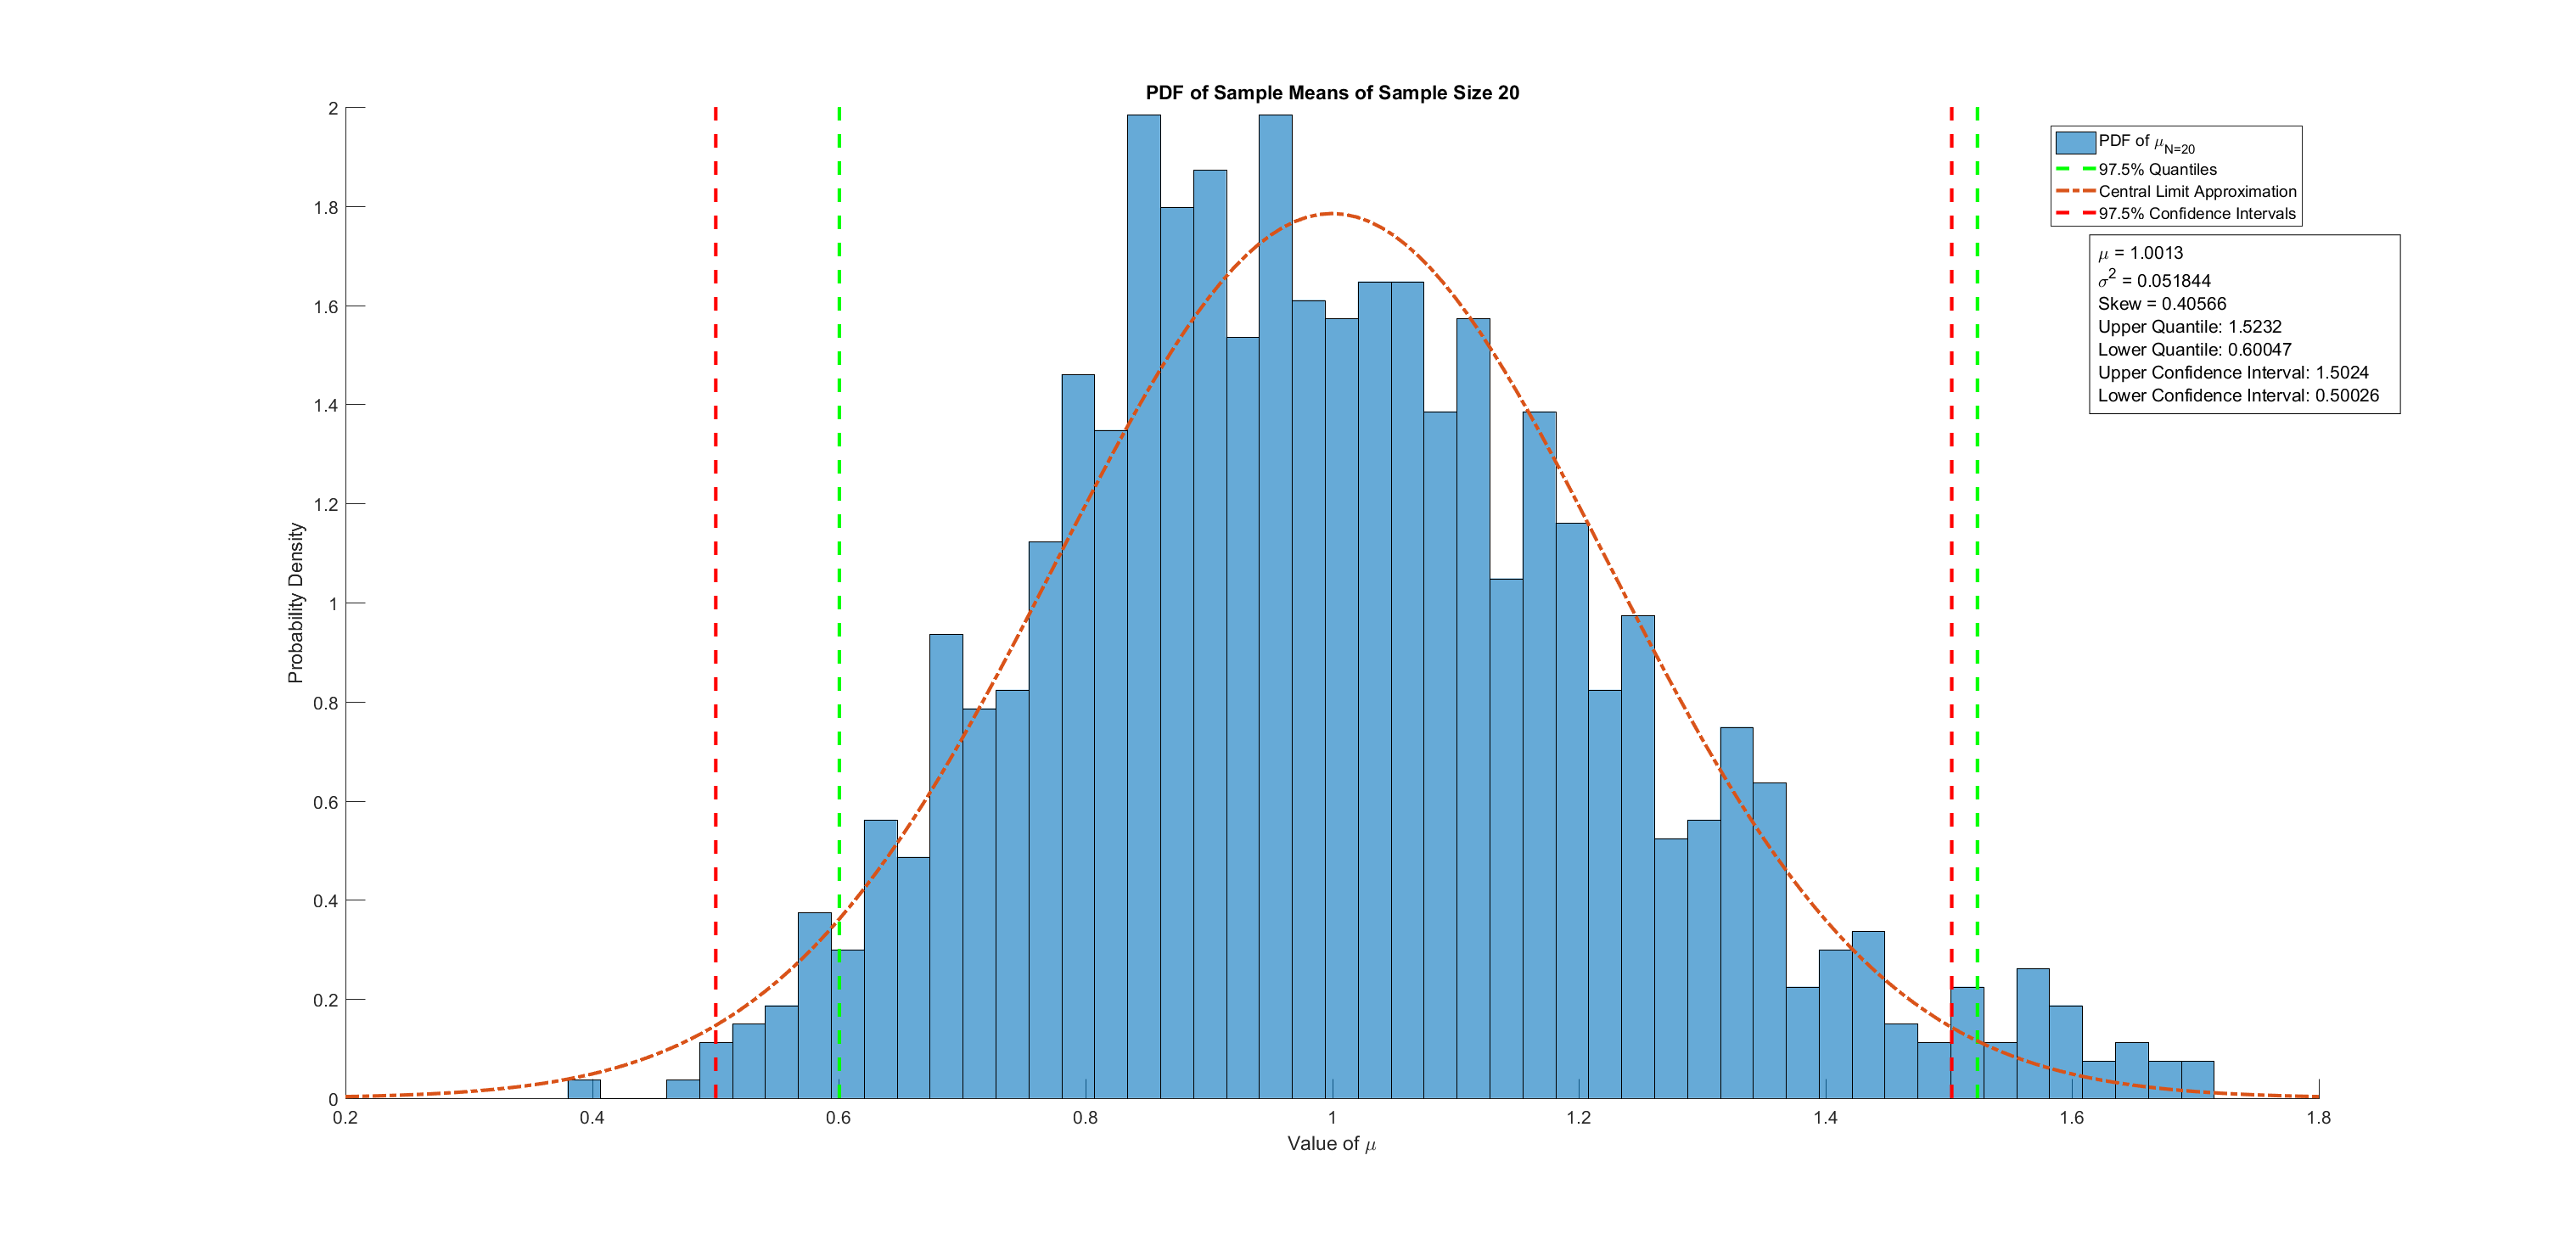
\includegraphics [width=4in]{prob4_03.eps}

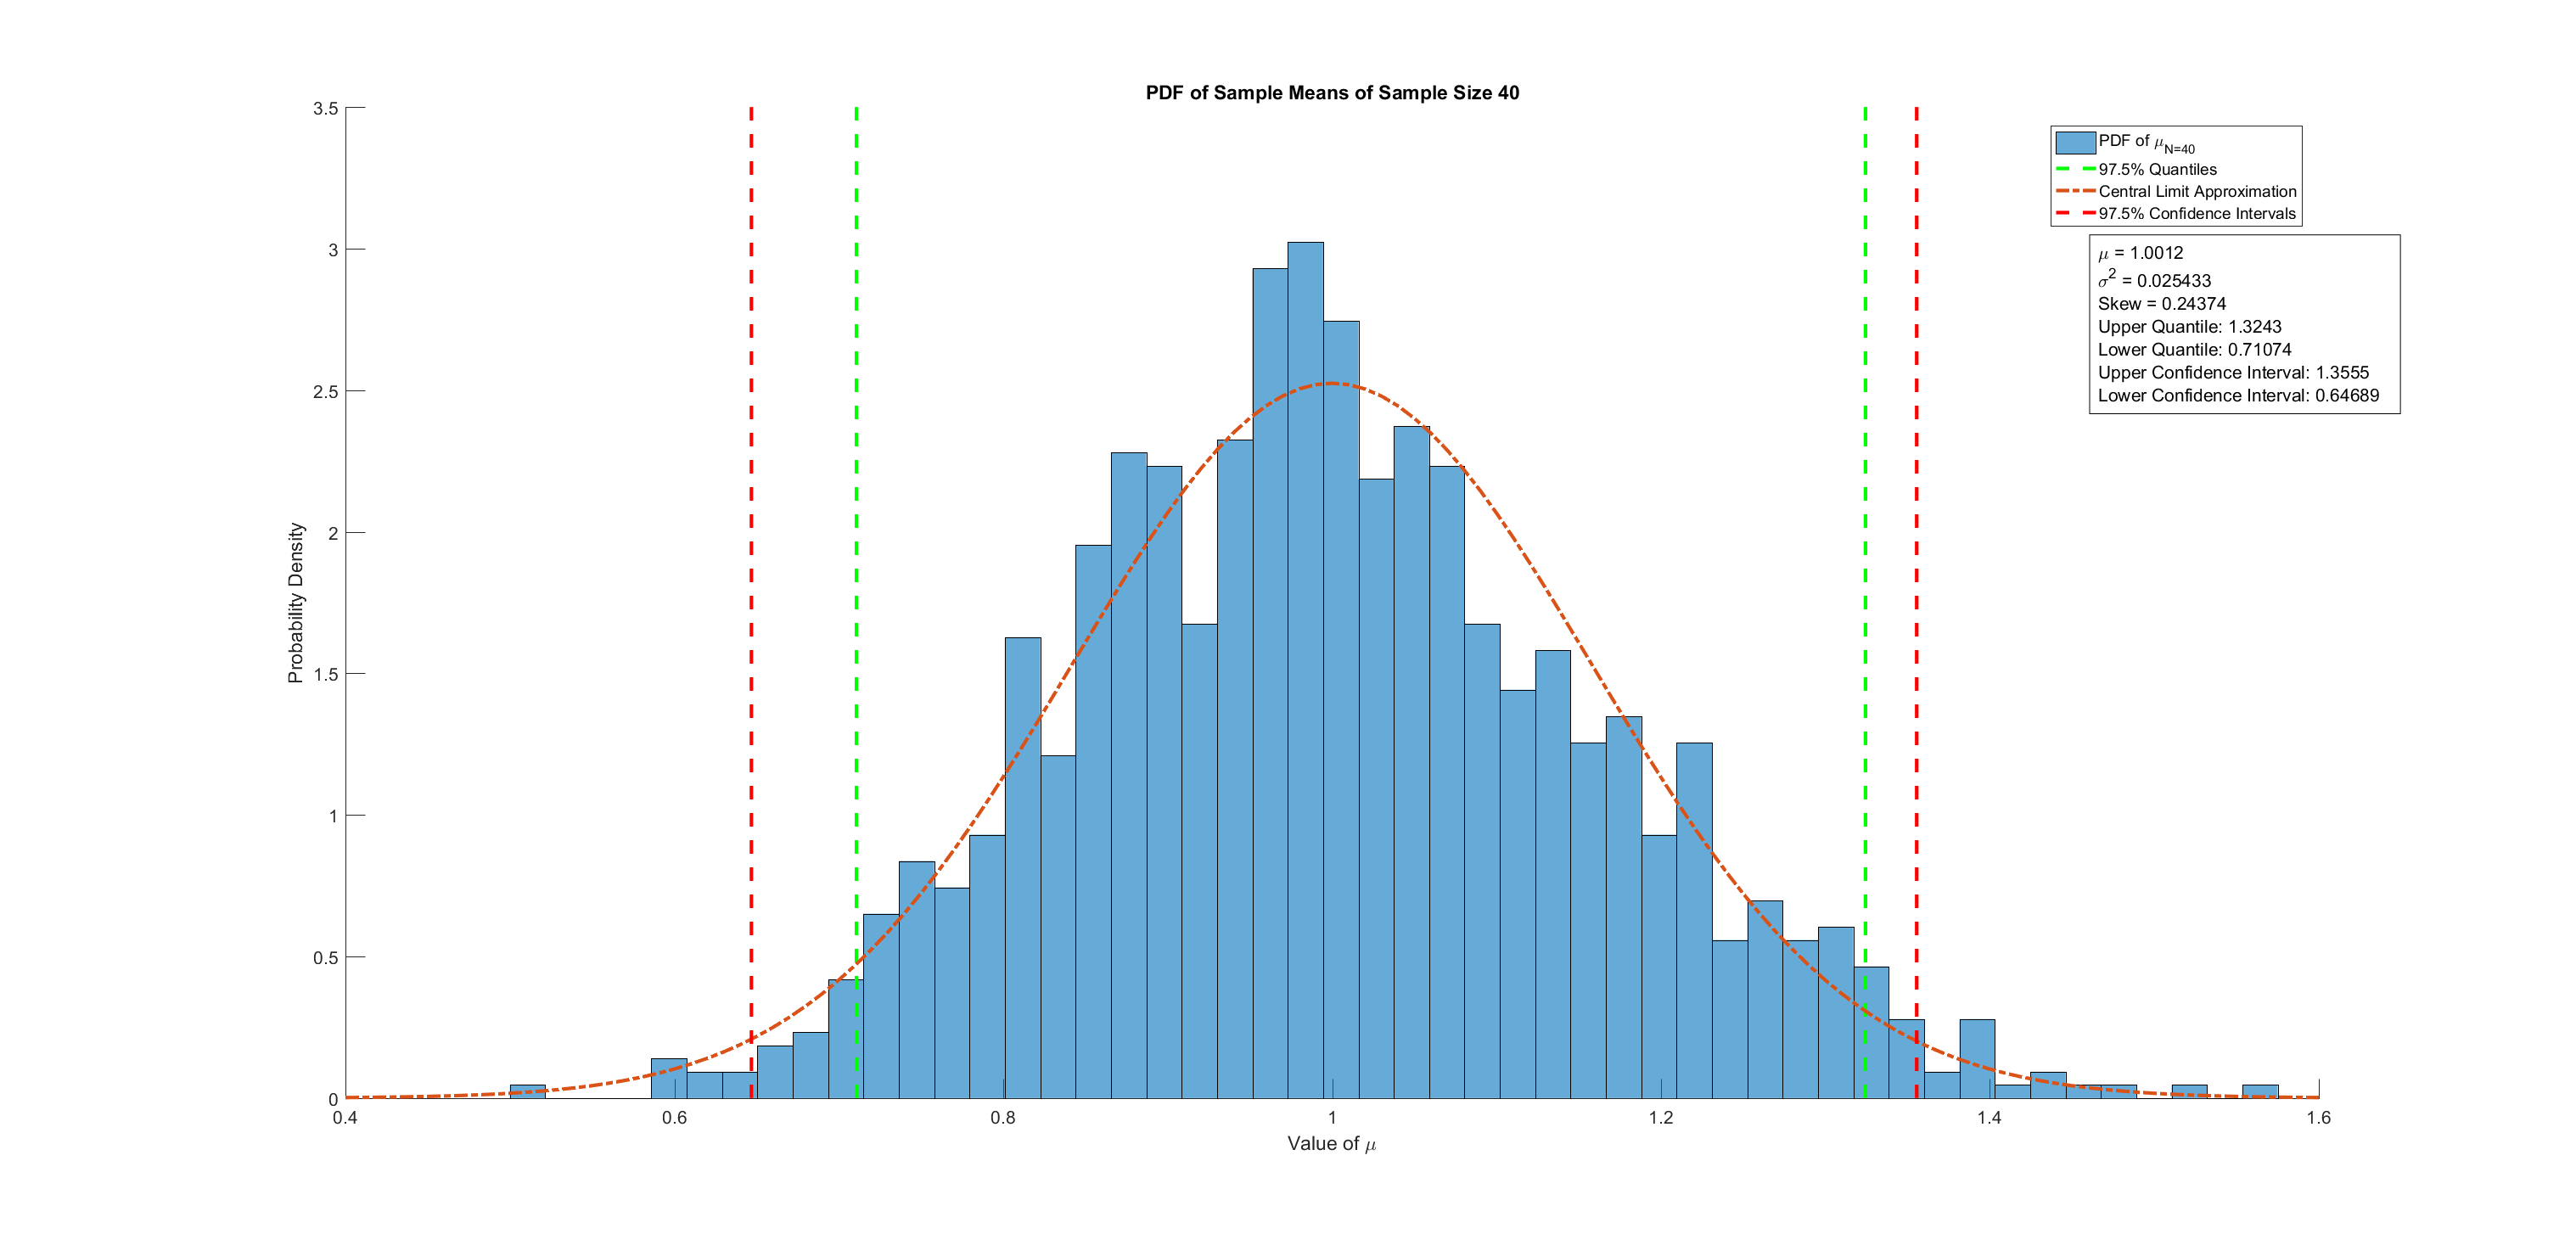
\includegraphics [width=4in]{prob4_04.eps}

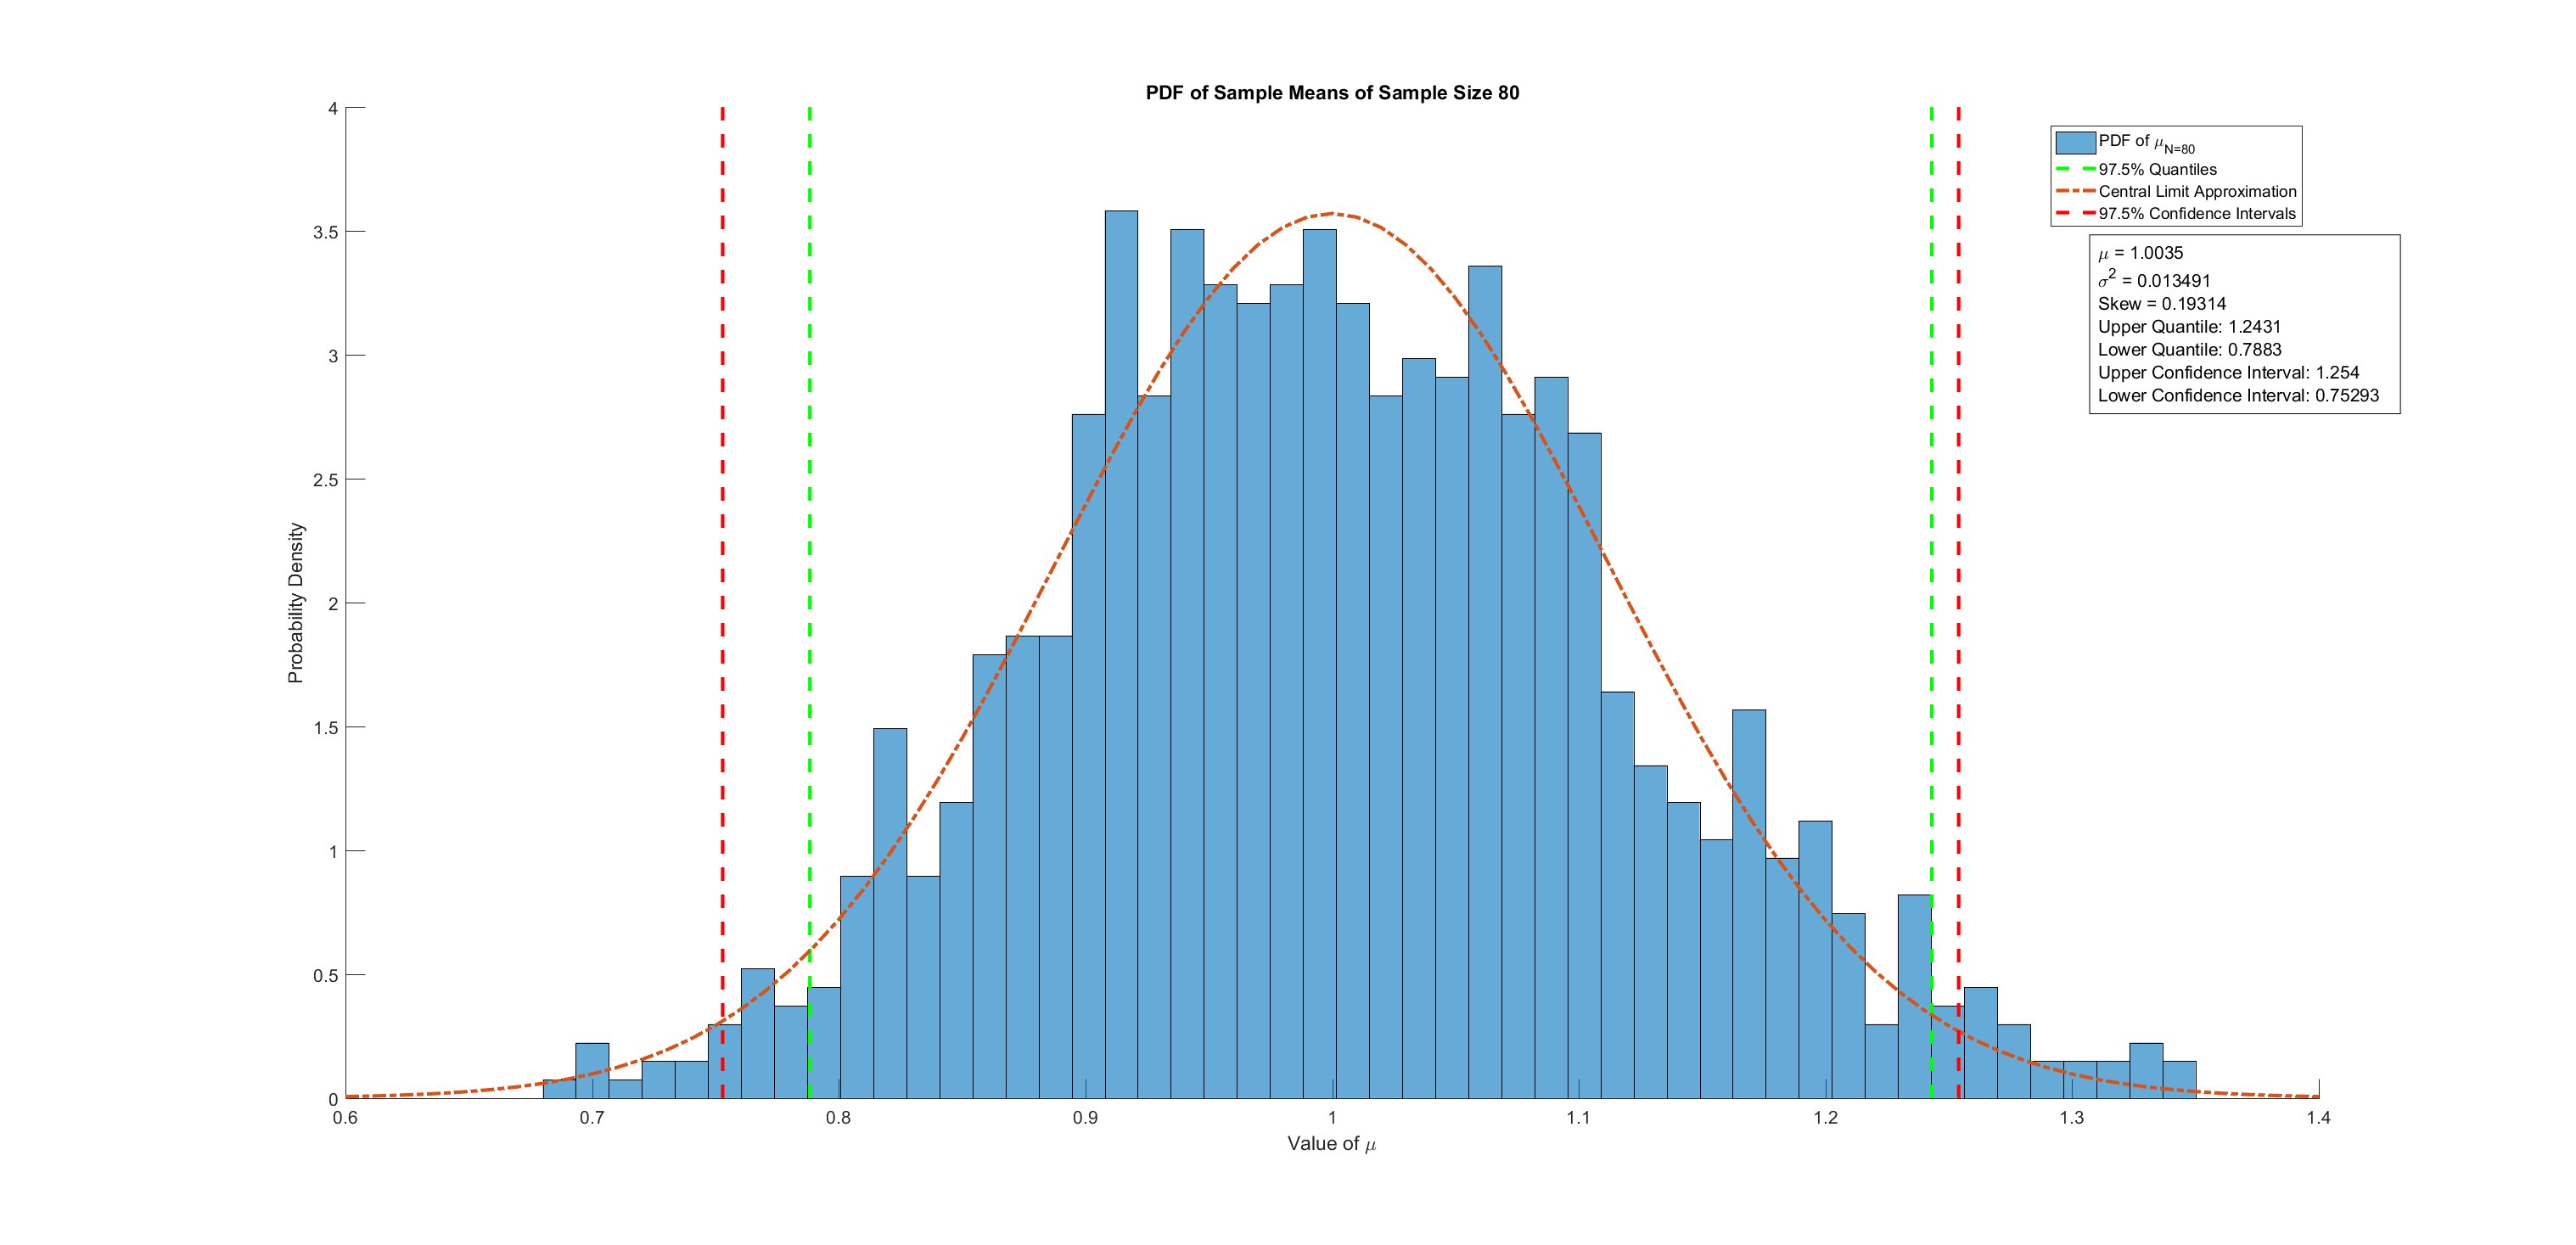
\includegraphics [width=4in]{prob4_05.eps}

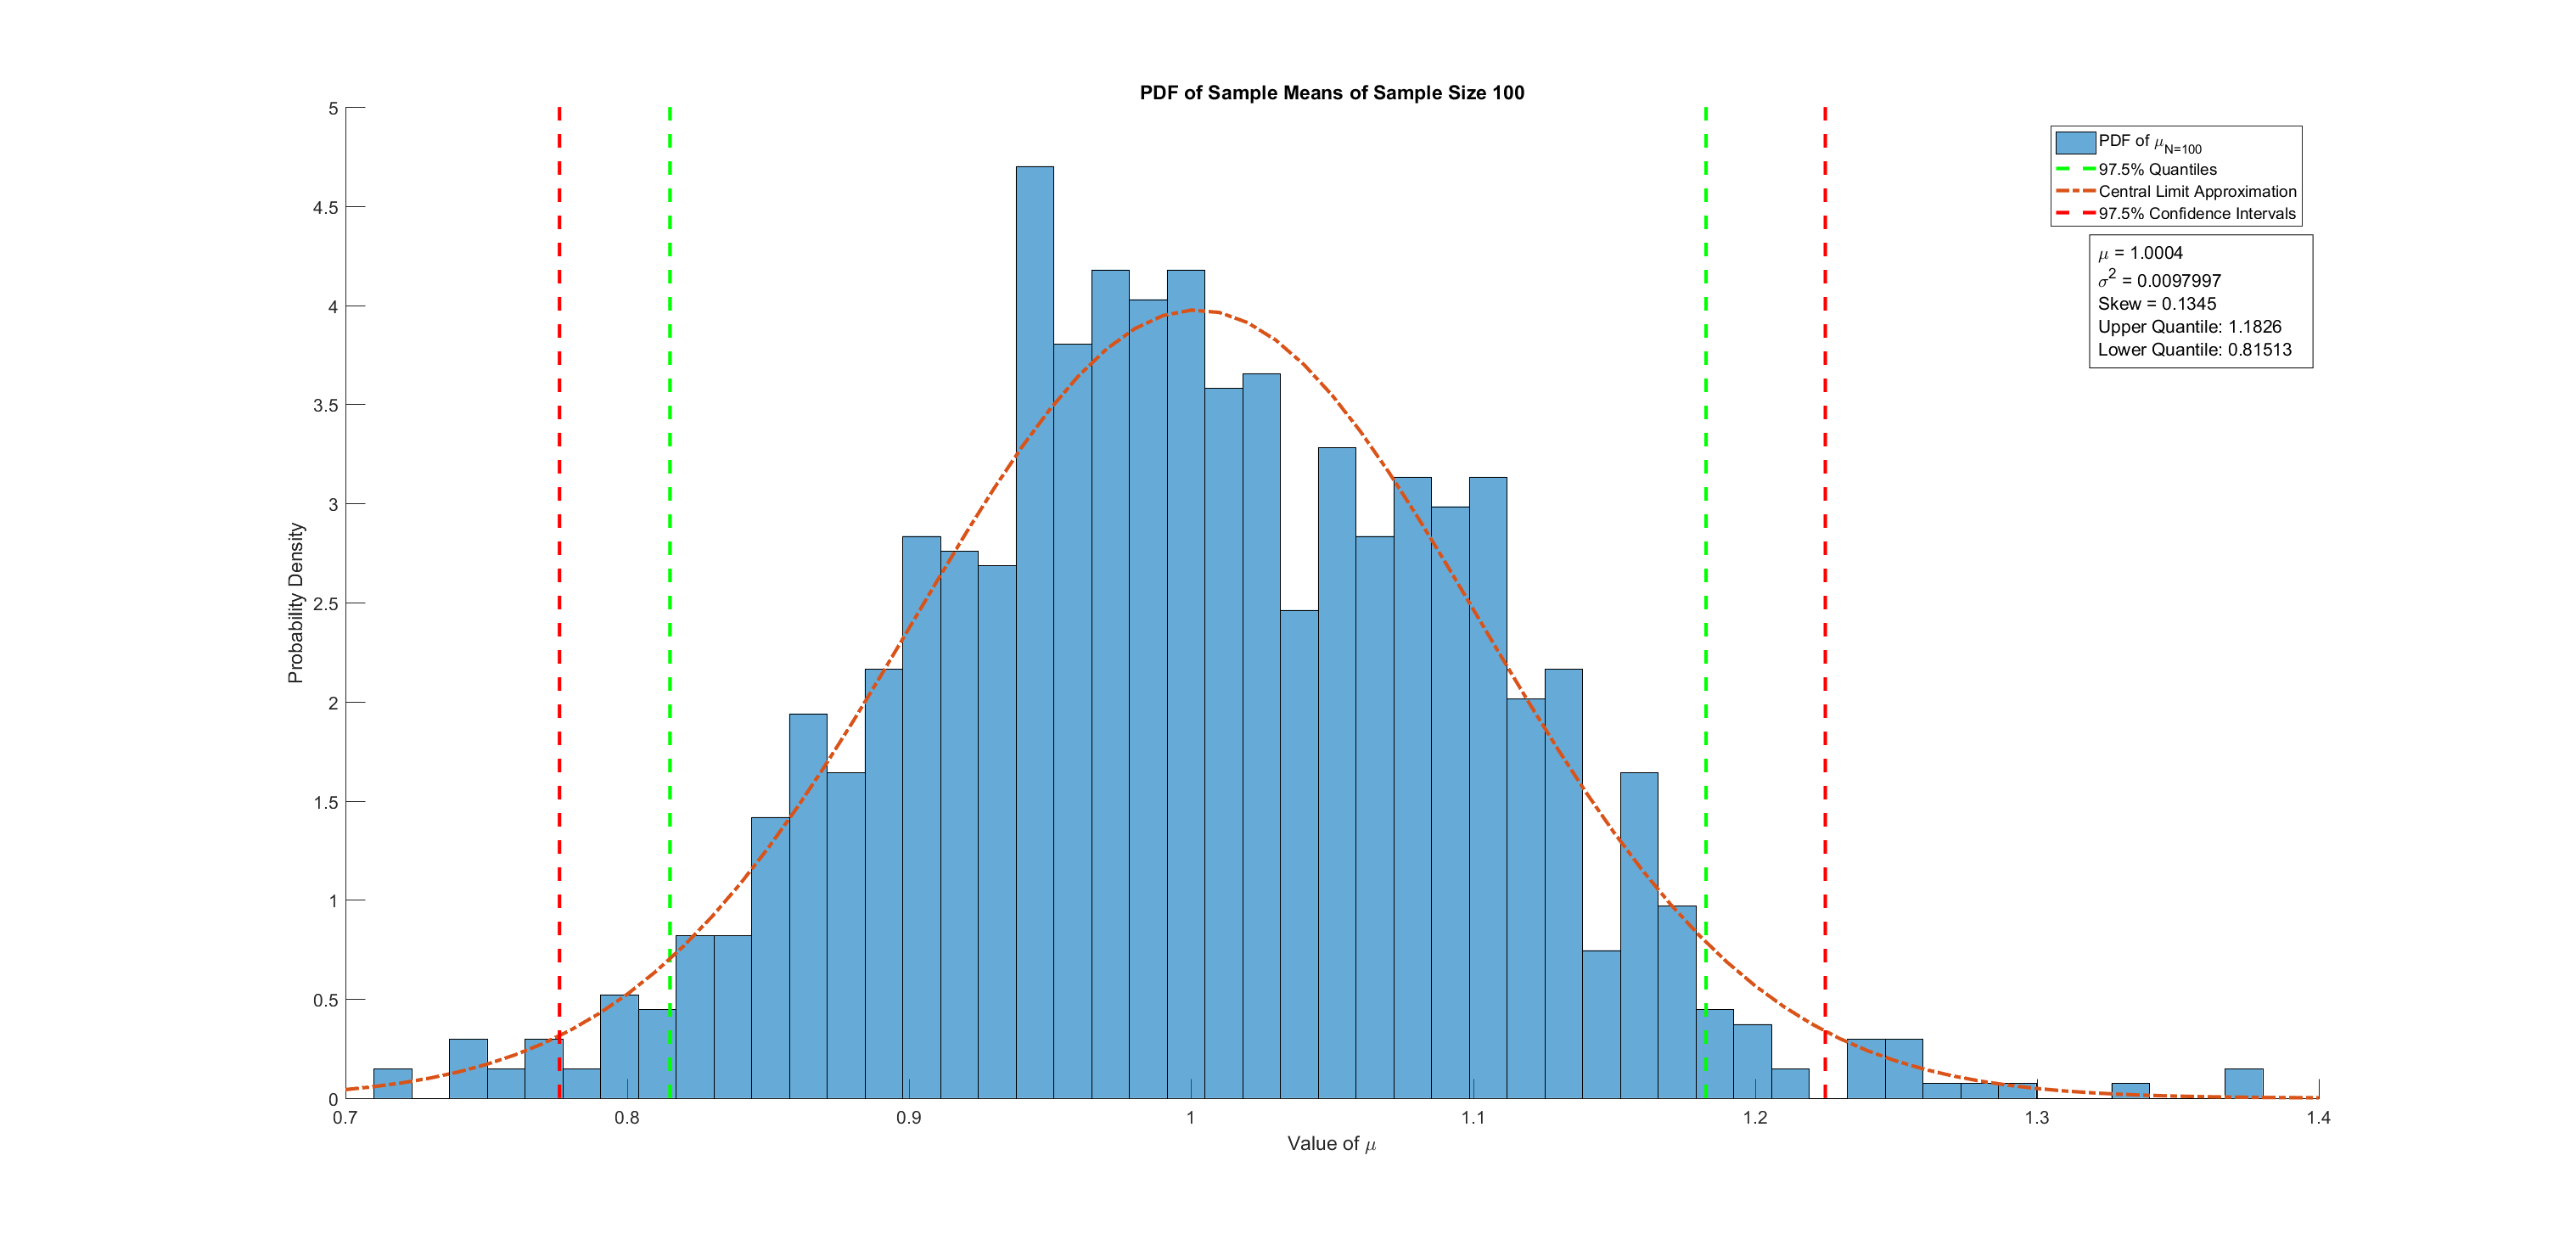
\includegraphics [width=4in]{prob4_06.eps}

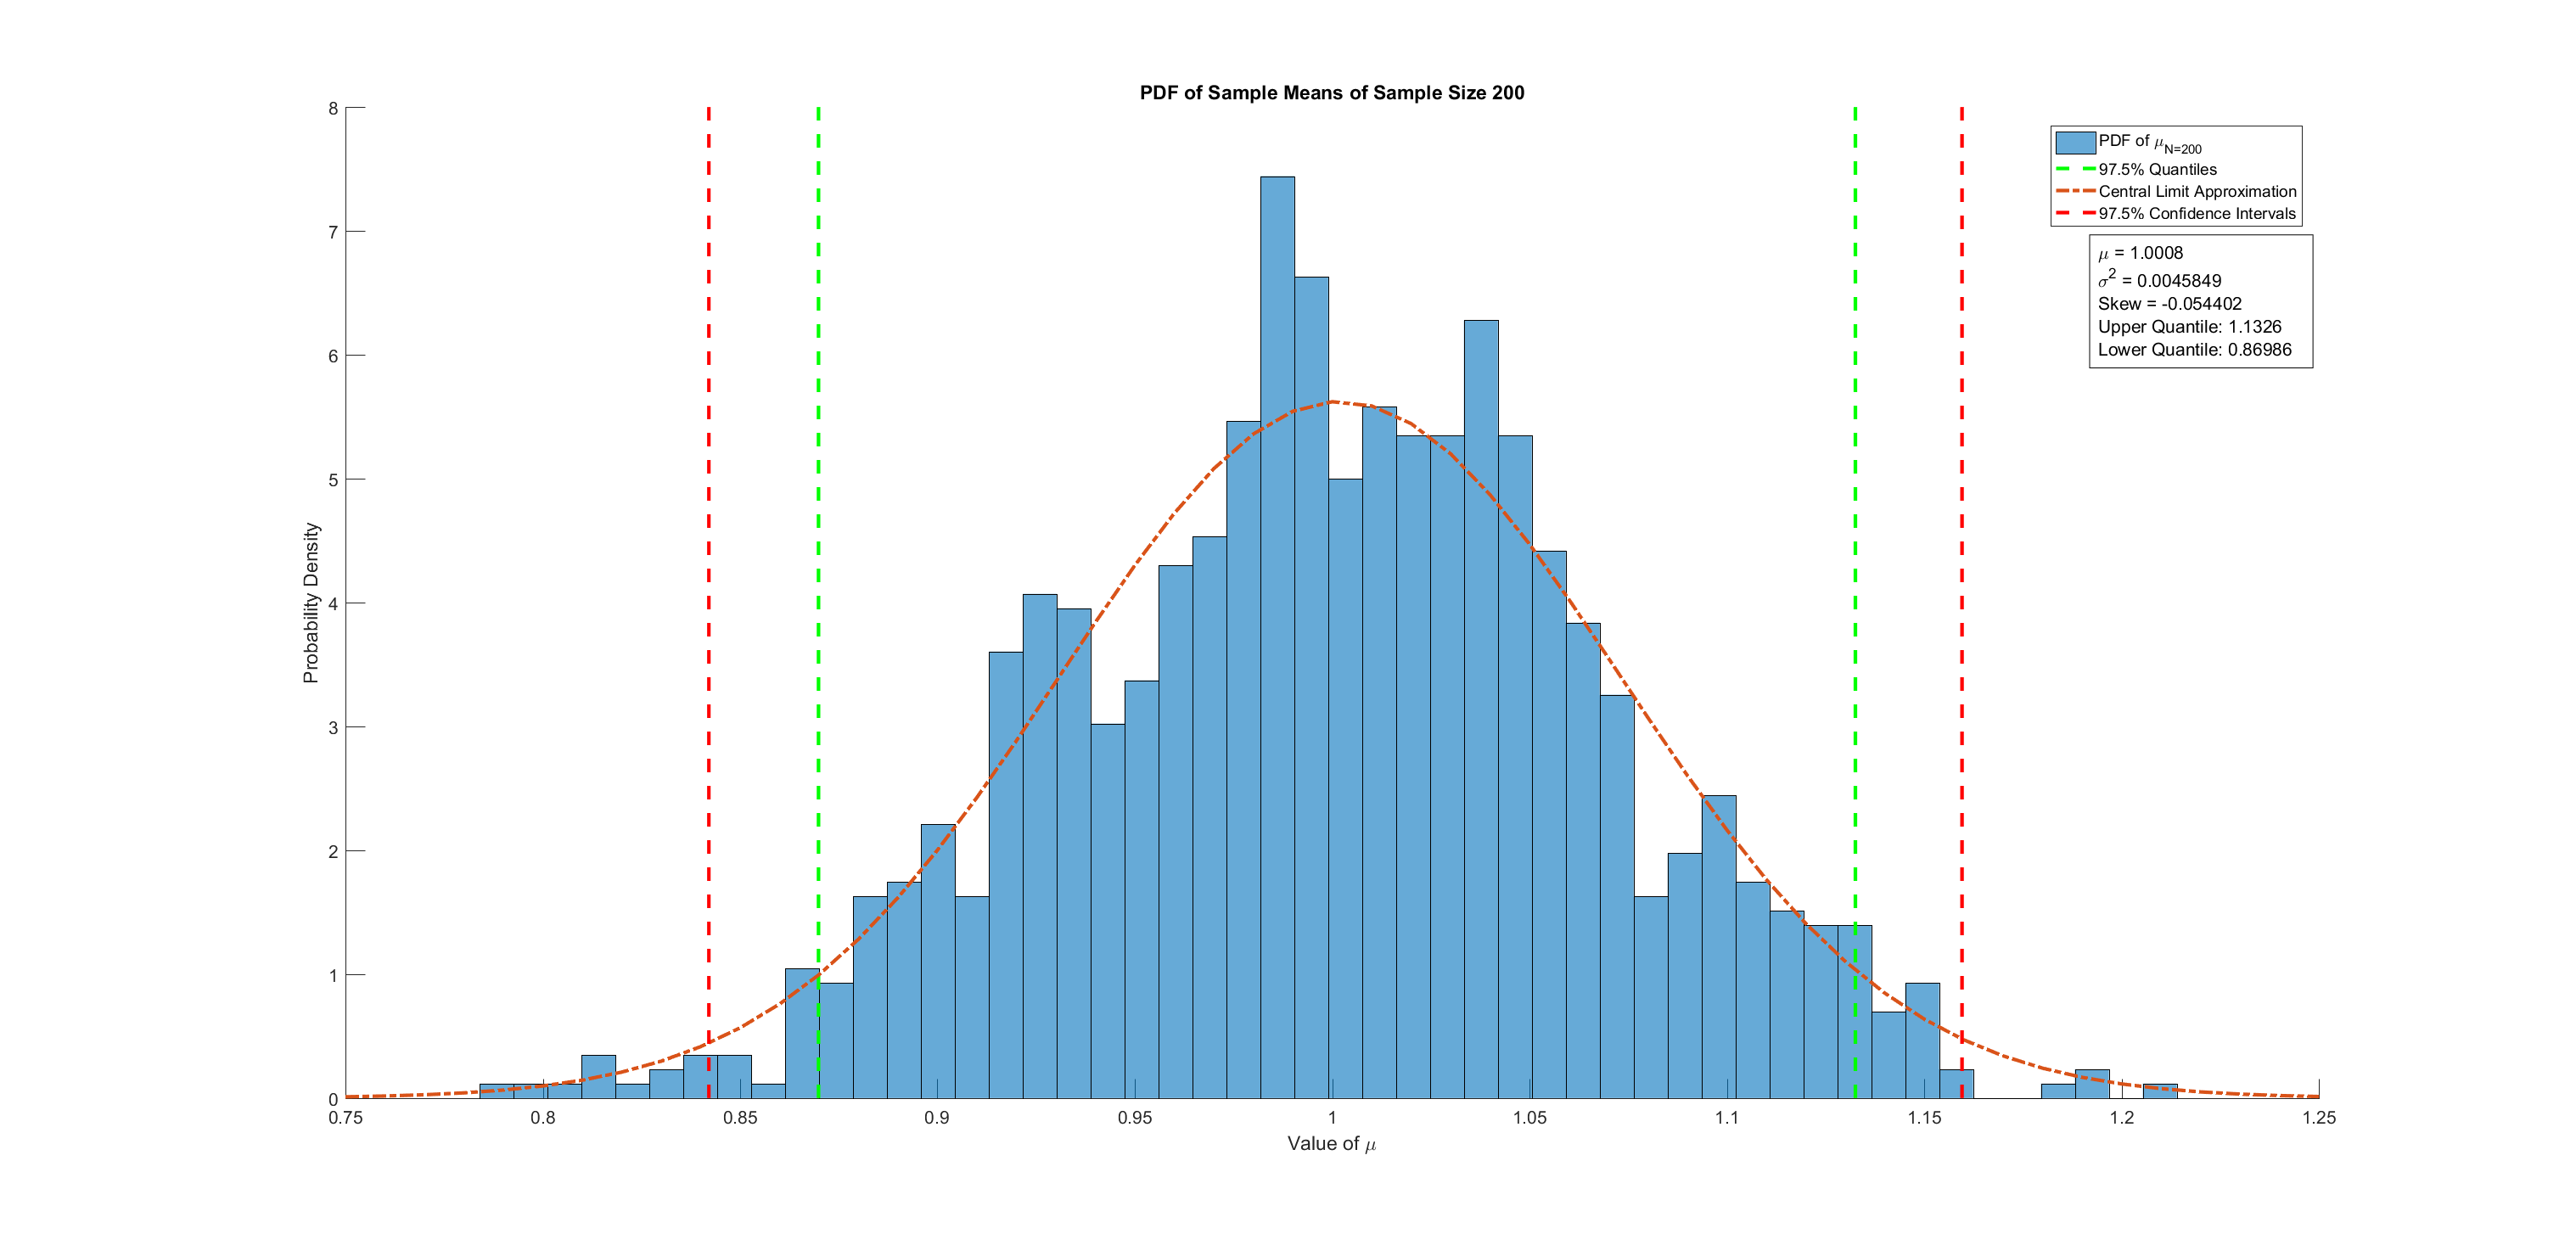
\includegraphics [width=4in]{prob4_07.eps}

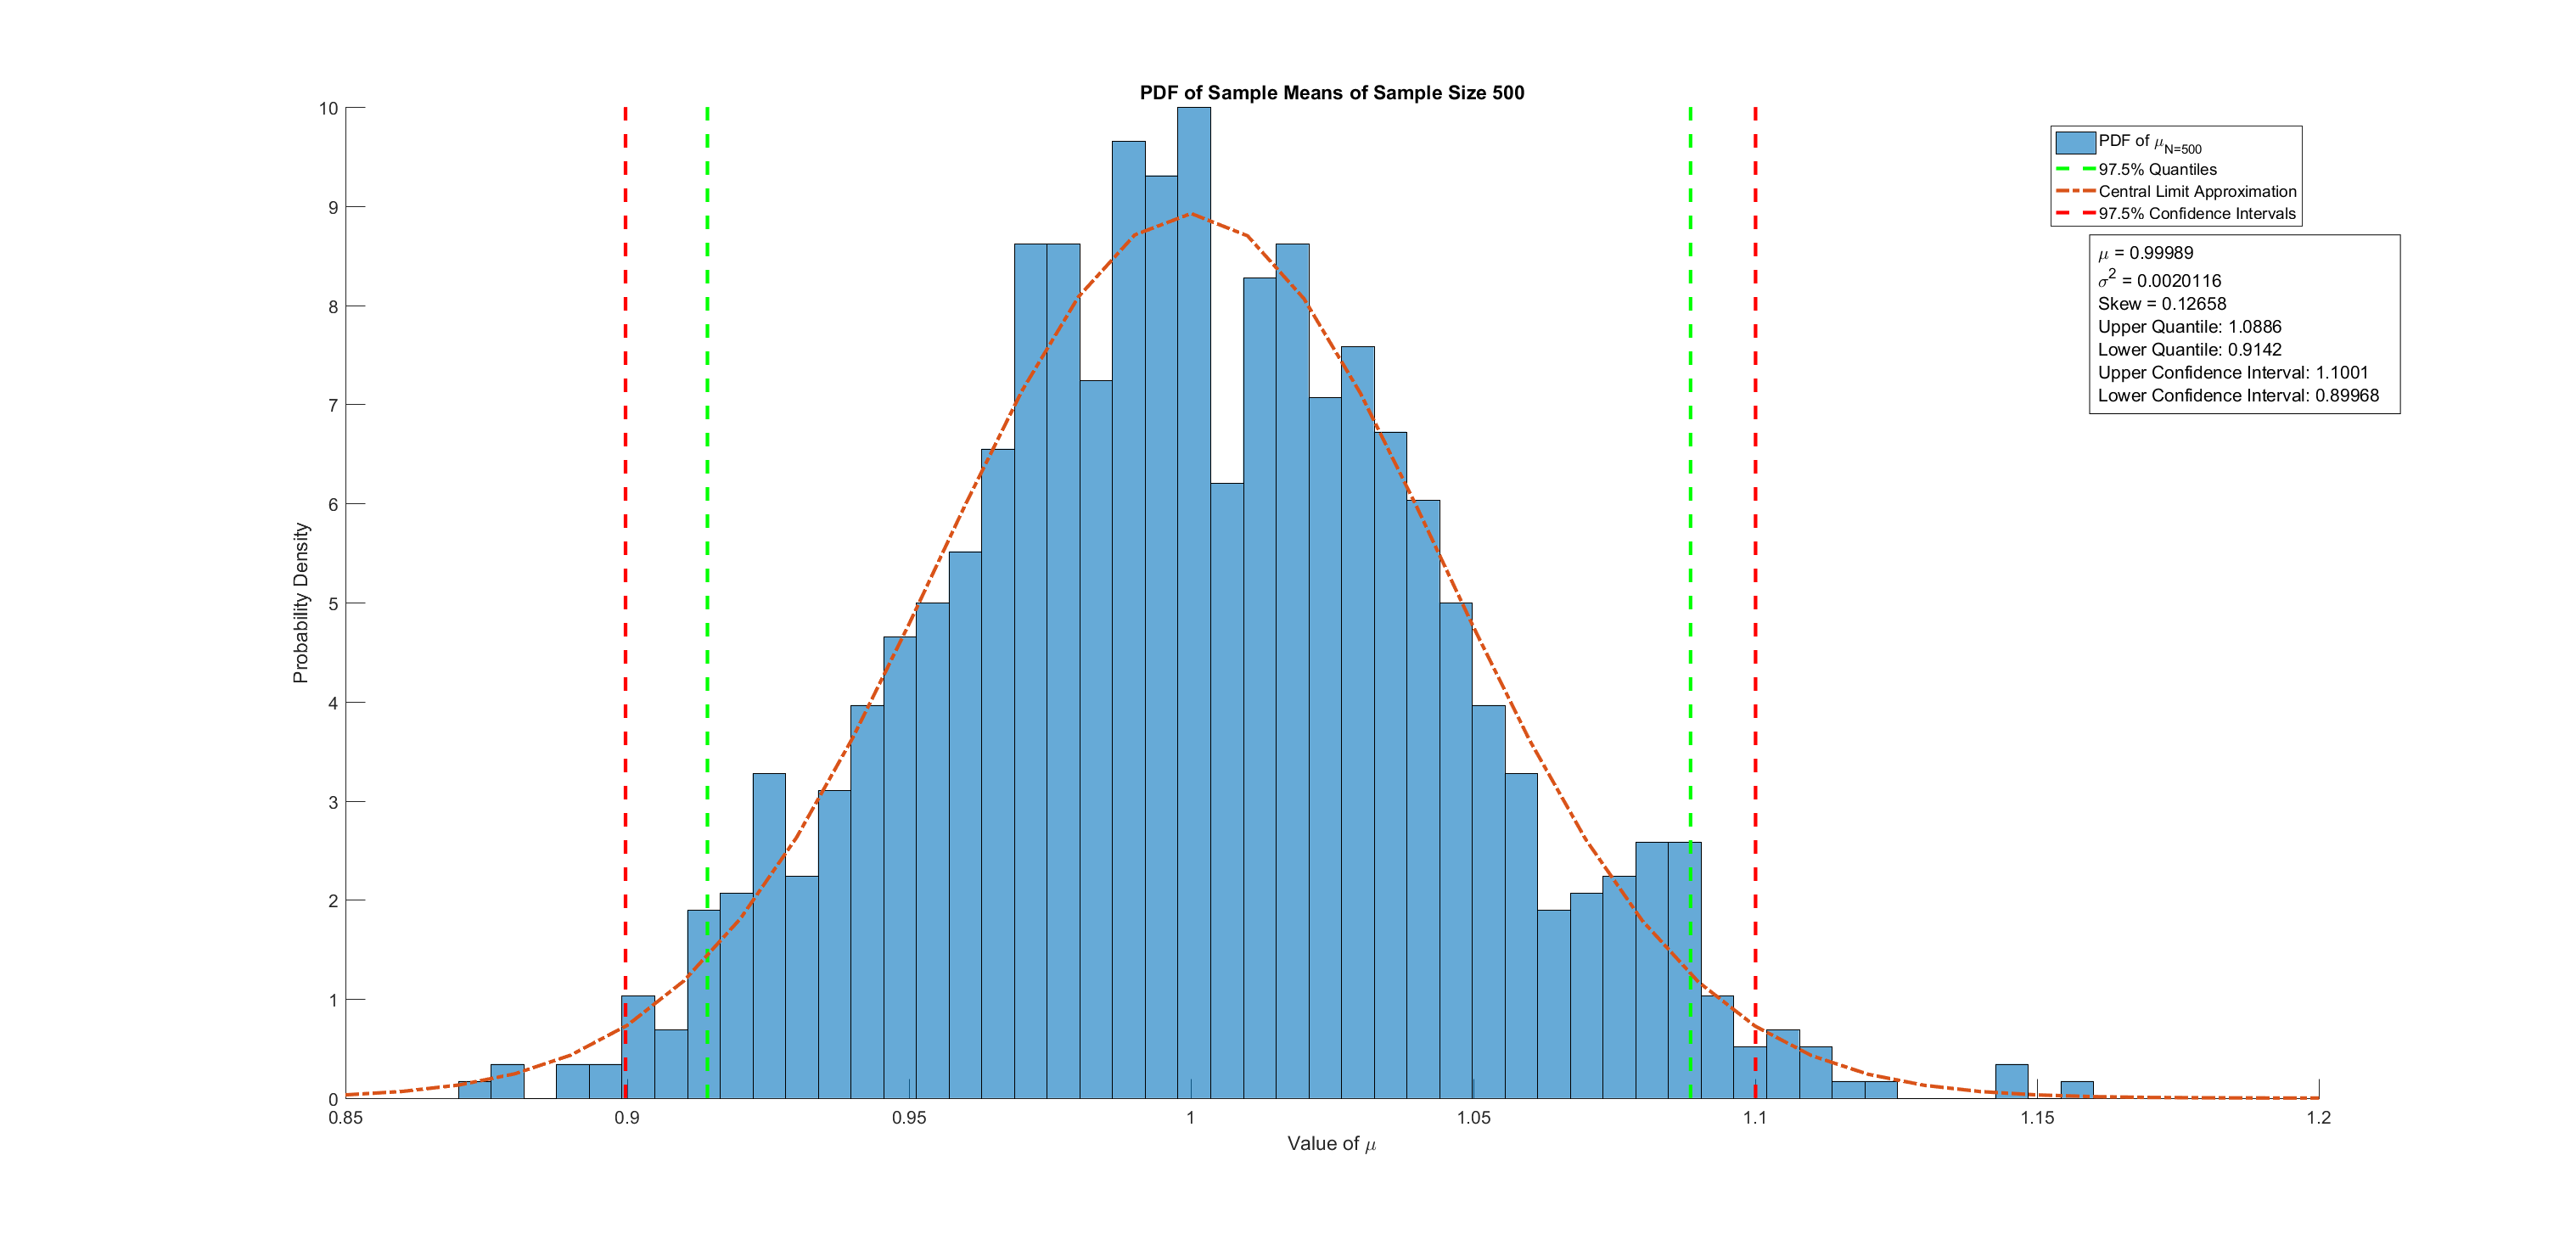
\includegraphics [width=4in]{prob4_08.eps}



\end{document}
    
